\documentclass[
    12pt,
    a4paper,
    addpoints,
    answers,
    convocatoria=ord,
    titulacion=CD,
    curso=2024/2025,
]{db-exam}

\begin{document}

\begin{questions}

\question[3] \textbf{Modelado conceptual}

Queremos guardar información sobre estructuras cerebrales. Estas estructuras están formadas por neuronas, identificadas por un id único. Además, pueden tener asociada una única función de activación (de momento ReLU, sigmoide y tangente hiperbólica).

Dentro de una misma estructura, cada neurona tiene que estar conectada al menos a otra neurona que pertenezca a la misma estructura, estando cada una de estas conexiones caracterizada por un peso. Eso sí, dentro de una misma estructura dos neuronas solo se pueden conectar una única vez entre ellas.

Podemos tener diferentes estructuras cerebrales, cada una identificada por un nombre único y una descripción, y las neuronas pueden pertenecer a diferentes estructuras a la vez (como mínimo a una), si bien cada par conectado debe estar dentro de la misma estructura.

\begin{itemize}
    \item Realiza un modelo conceptual de datos mediante la técnica del modelo entidad-relación de Chen que modele el sistema descrito.
    \item Realiza el paso a tablas del diagrama que has propuesto.
\end{itemize}

\begin{solution}

\begin{center}
    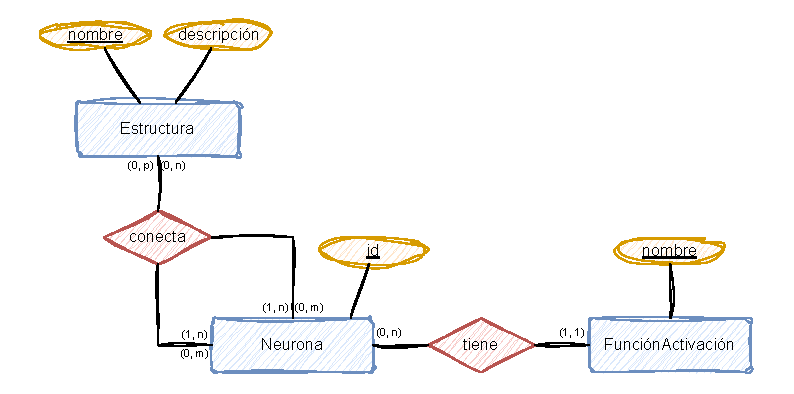
\includegraphics[width=\textwidth]{examenes/figs/bbdd-gcdia-2024-2025-ordinaria-er.pdf}
\end{center}

\begin{center}
    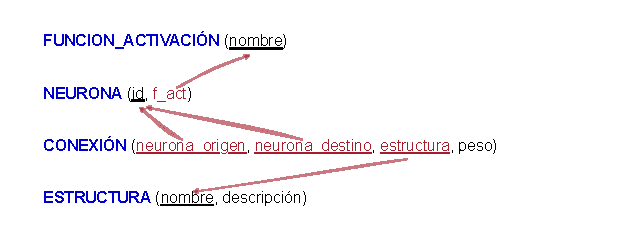
\includegraphics[width=\textwidth]{examenes/figs/bbdd-gcdia-2024-2025-ordinaria-tablas.pdf}
\end{center}

\end{solution}

\question[5] \textbf{Álgebra relacional y SQL}

Supón que estamos modelando un perceptrón multicapa. Este está formado por varias capas (una de entrada, una de salida y varias ocultas), cada capa contiene varias neuronas y las conexiones siempre van de una capa a la siguiente. Además las capas tienen un orden, que viene definido por una posición que indica su posición en la red.

\texttt{CAPA (\underline{id\_c}, tipo, pos)} - \texttt{NEURONA (\underline{id}, \underline{id\_c}, f\_act)} - \texttt{ENLACE (\underline{capa\_from}, \underline{capa\_to}, peso)}
    
Se pide:

\begin{parts}

\part[1] Álgebra relacional
\begin{subparts}

\subpart[\half] Describe con tus propias palabras los siguientes operadores: producto cartesiano, intersección, diferencia, división y proyección.

\begin{solution}[7.5em]

\begin{itemize}
    \item Producto cartesiano ($\times$): Combina cada tupla de una relación con todas las tuplas de otra.
    \item Intersección ($\cap$): Devuelve las tuplas comunes a dos relaciones.
    \item Diferencia ($-$): Devuelve las tuplas que están en la primera relación pero no en la segunda.
    \item División ($\div$): Devuelve los elementos de una relación que están relacionados con todos los elementos de otra relación.
    \item Proyección ($\Pi$): Selecciona columnas específicas de una relación.
\end{itemize}

\end{solution}

\subpart[\half] Expresa en álgebra relacional la consulta que obtiene los identificadores de las neuronas que pertenecen a capas de tipo \enquote{oculta} y cuya función de activación es \enquote{ReLU}.

\begin{solution}[7.5em]

$$
\Pi_{id_c}(\sigma_{f\_act=\text{\enquote{ReLU}}}(NEURONA) \bowtie \sigma_{tipo=\text{\enquote{oculta}}}(CAPA))
$$

\end{solution}

\end{subparts}
    
\part[2] Consultas SQL

\begin{subparts}

\subpart[\half] Obtener los id de todas aquellas capas de tipo \enquote{oculta} que no tienen ningún enlace entrante.

\begin{solution}[6em]

\begin{lstlisting}[language=sql]
SELECT id_c
FROM CAPA
WHERE tipo = 'oculta'
  AND id_c NOT IN (SELECT capa_to FROM ENLACE);
\end{lstlisting}

\end{solution}

\subpart[\half] Obtener el número total de neuronas que hay en la capa de salida.

\begin{solution}[6em]

\begin{lstlisting}[language=sql]
SELECT COUNT(*)
FROM NEURONA
WHERE id_c IN (SELECT id_c FROM CAPA WHERE tipo = 'salida');
\end{lstlisting}

o

\begin{lstlisting}[language=sql]
SELECT COUNT(DISTINCT id)
FROM NEURONA n
JOIN CAPA c ON c.id = n.ic_c
WHERE tipo = 'salida';
\end{lstlisting}

\end{solution}

\subpart[\half] Obtener los id de las capas cuya suma total de pesos de los enlaces salientes sea negativa.

\begin{solution}[6em]

\begin{lstlisting}[language=sql]
SELECT capa_from 
FROM ENLACE 
GROUP BY capa_from 
HAVING SUM(peso) < 0;
\end{lstlisting}

\end{solution}

\subpart[\half] Obtener los id de aquellas neuronas ocultas cuya función de activación sea «sigmoide».

\begin{solution}[6em]

\begin{lstlisting}[language=sql]
SELECT id
FROM NEURONA
WHERE f_act = 'sigmoide'
  AND id_c IN (SELECT id_c FROM CAPA WHERE tipo = 'oculta');
\end{lstlisting}

o

\begin{lstlisting}[language=sql]
SELECT n.id 
FROM NEURONA n
JOIN CAPA c ON c.id = n.id_c
WHERE n.f_act = 'sigmoide'
  AND c.tipo = 'oculta';
\end{lstlisting}

\end{solution}

\end{subparts}

\part[1] Escribe un \textit{trigger} que impida insertar un enlace cuya capa de origen no sea inmediatamente anterior a la capa de destino.

\begin{solution}[34em]

\begin{lstlisting}[language=sql]
DELIMITER $$

CREATE TRIGGER validar_enlace
BEFORE INSERT ON ENLACE
FOR EACH ROW
BEGIN
  DECLARE pos_from INT;
  DECLARE pos_to INT;

  SELECT pos INTO pos_from FROM CAPA WHERE id_c = NEW.capa_from;
  SELECT pos INTO pos_to FROM CAPA WHERE id_c = NEW.capa_to;

  IF pos_to <> pos_from + 1 THEN
    SIGNAL SQLSTATE '7291'
    SET MESSAGE_TEXT = 'Las capas no son consecutivas';
  END IF;
END;
$$

DELIMITER ;
\end{lstlisting}

\end{solution}

\part[1] Escribe un procedimiento almacenado que, dado el id de una capa oculta (comprobarlo), devuelva el número de enlaces entrantes y salientes (por separado) que tiene.

\begin{solution}

\begin{lstlisting}[language=sql]
DELIMITER $$

CREATE PROCEDURE contar_enlaces_oculta(
    IN id_capa INT,
    OUT num_entrantes INT,
    OUT num_salientes INT
)
BEGIN
  DECLARE tipo_capa VARCHAR(20);

  SELECT tipo INTO tipo_capa
  FROM CAPA
  WHERE id_c = id_capa;

  IF tipo_capa = 'oculta' THEN
    SELECT COUNT(*) INTO num_entrantes
    FROM ENLACE
    WHERE capa_to = id_capa;

    SELECT COUNT(*) INTO num_salientes
    FROM ENLACE
    WHERE capa_from = id_capa;
  ELSE
    SIGNAL SQLSTATE '7291'
    SET MESSAGE_TEXT = 'La capa tiene que ser oculta';
  END IF;
END;
$$

DELIMITER ;
\end{lstlisting}

\end{solution}

\end{parts}

\question[2] \textbf{Programación contra bases de datos.}

Tomando como punto de partida un esquema \textbf{basado} en el modelo relacional anterior (el del bloque 2), completa los huecos (marcados con \texttt{TODO} del siguiente código fuente en Python de tal manera que se satisfaga la funcionalidad indicada en los \textit{docstrings}.

\begin{lstlisting}[language=Python]
import mysql.connector

conn = mysql.connector.connect(
    host="nasa.gov",
    user="romualdo",
    password="RuPauL.Dr4gR4c3",
    database="redes_neuronales"
)
cursor = conn.cursor()

def obtener_neuronas_capa(pos):
    """Obtiene las neuronas de una capa dada su posición en la red.

    :param pos: La posición de la capa dentro de la red:
    :return: Una lista con los id y las funciones de activación de
        las neuronas.
    """
    # TODO
\end{lstlisting}

\begin{solutionorbox}
\begin{lstlisting}[language=Python]
    consulta = """
    SELECT NEURONA.id, NEURONA.f_act
    FROM NEURONA
    JOIN CAPA ON NEURONA.id_c = CAPA.id_c
    WHERE CAPA.pos = %s;
    """
\end{lstlisting}
\end{solutionorbox}

\begin{lstlisting}[language=Python]
    cursor.execute(consulta, (id_capa,))
    return cursor.fetchall()

def insertar_enlace(id_capa_origen, id_capa_destino, peso):
    """Añade un nuevo enlace entre dos capas consecutivas.
    
    :param id_capa_origen: La capa de origen.
    :param id_capa_destino: La capa destino.
    :param El peso a asignar a toda las neuronas de las dos capas
    :return: True si las capas son consecutivas y se ha insertado el
        enlace o False en caso contrario
    """
    # TODO
\end{lstlisting}

\begin{solutionorbox}
\begin{lstlisting}[language=Python]
    cursor.execute("SELECT pos FROM CAPA WHERE id_c = %s", (id_capa_origen,))
    pos_origen = cursor.fetchone()[0]

    cursor.execute("SELECT pos FROM CAPA WHERE id_c = %s", (id_capa_destino,))
    pos_destino = cursor.fetchone()[0]

    if pos_destino == pos_origen + 1:
        cursor.execute(
            "INSERT INTO ENLACE (capa_from, capa_to, peso)
                         VALUES (%s, %s, %s)",
            (id_capa_origen, id_capa_destino, peso)
        )
        conn.commit()
        return True
    return False
\end{lstlisting}
\end{solutionorbox}

\begin{lstlisting}[language=Python]
\begin{solutionorbox}

def capas_sin_enlaces_salientes():
    """Lista todas las capas que no tienen ningun enlace saliente.

    :return: Lista con los id de las capas, ordenadas por posición.
    """
    # TODO
\end{lstlisting}

\begin{solutionorbox}
\begin{lstlisting}[language=Python]
    consulta = """
    SELECT id_c
    FROM CAPA
    WHERE id_c NOT IN (SELECT capa_from FROM ENLACE)
    ORDER BY pos;
    """
\end{lstlisting}
\end{solutionorbox}

\begin{lstlisting}[language=Python]
    cursor.execute(consulta)
    return cursor.fetchall()

conn.close()
\end{lstlisting}



\end{questions}
\end{document}